\documentclass{beamer}

\usetheme[compactlogo,white]{Madison}
\usefonttheme[onlymath]{serif}

\usepackage{amsmath}
\usepackage{amssymb,amsfonts,amsthm}
\usepackage{graphicx}
\graphicspath{{figs/}}
\usepackage{natbib}
% \usepackage{caption}
% \captionsetup[figure]{font=small}

\begin{document}

\small

\begin{frame}{Problem}
    \begin{itemize}
        \item Consider: want to model the probability a pitch will be called a strike given the game situation, personnel involved, and the location of the pitch
        \begin{figure}
            \centering
            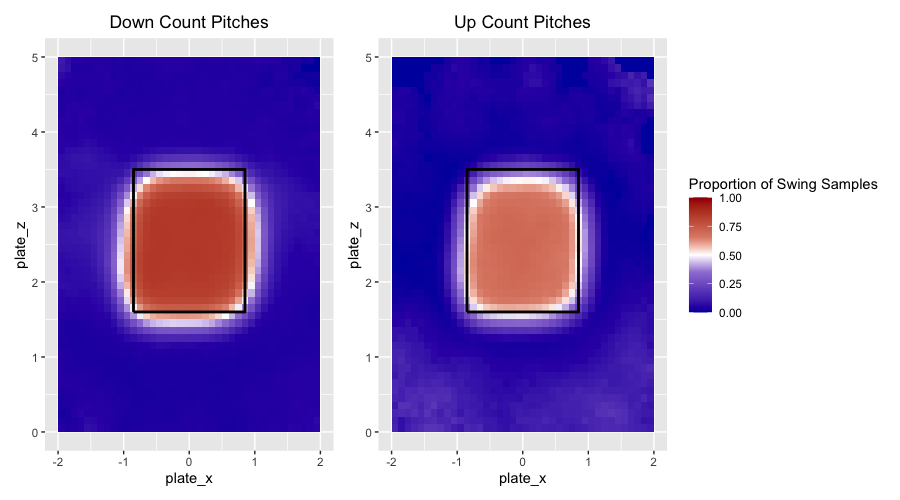
\includegraphics[width=.5\textwidth]{counts.png}
            \caption{Example of strike probability surface for different game situations}
        \end{figure}
        \item Currently, we use a standard implementation of BART probit to estimate the probability a pitch will be called a strike which presents several issues:
        \begin{itemize}
            \item Discrete nature of BART makes it difficult to determine how changes in pitch location influence strike probability
            \item Computation and prediction may be slower due to larger trees
        \end{itemize}
    \end{itemize} 
\end{frame}

\begin{frame}{Proposal}
    \begin{itemize}
        \item Implement BART with a spatially adaptive Bayesian p-spline at the node level
        \begin{itemize}
            \item This will allow better inference to be made about how changes in location effect the strike probability, since the output will be a smooth probability surface
            \item It could also potentially improve computation speed, since we may be able to use fewer and smaller trees to achieve similar results as a standard BART implementation
        \end{itemize}
        \item Use a randomization technique to speed up the computation, since the coefficients and log-likelihood for the spatially adaptive Bayesian p-spline must be calculated for each node, of each tree, for every sample
    \end{itemize} 
\end{frame}

\begin{frame}{Desired Results}
    \begin{itemize}
        \item Show that BART with a spatially adaptive Bayesian p-spline provides more accurate results than standard BART implementation for the strike problem
        \item Show that using a randomization technique improves the speed of BART with a spatially adaptive Bayesian p-spline without compromising results
        \item (Potentially) Show BART with a spatially adaptive Bayesian p-spline can compute faster and provide more accurate results than standard BART by using fewer trees
    \end{itemize} 
\end{frame}

\begin{frame}{Getting Desired Results}
    \begin{itemize}
        \item Work out necessary theoretical derivations for the model
        \item Implement the model in C++
        \begin{itemize}
            \item Sameer has a standard implementation of BART in C++ that I can use as a starting point
            \item I will need to update the inputs and the portions pertaining to drawing leaves
        \end{itemize}
        \item Run experiments to benchmark results against other implementations
    \end{itemize} 
\end{frame}

\begin{frame}{Next Steps}
    \begin{itemize}
        \item Read papers on BART and spatially adaptive Bayesian p-spline to start working out theoretical derivations
        \item Read papers to determine the most appropriate randomization technique to use for this problem
        \item Implement spatially adaptive Bayesian p-spline without BART (with and without randomization techniques)
        \item Continue to meet with Sameer
    \end{itemize} 
\end{frame}

\end{document}